
\documentclass{article}

\usepackage{tabularx,booktabs}
\usepackage{url}
% For basic math, align, fonts, etc.
\usepackage{amsmath}
\usepackage{amsthm}
\usepackage{amssymb}
\usepackage{mathtools}
\usepackage{mathrsfs}
\mathtoolsset{showonlyrefs}

\usepackage{hyperref}
\usepackage{siunitx}
\usepackage{float}
\usepackage{listings}

% For color
\usepackage{xcolor}
\definecolor{dark-red}{rgb}{0.4,0.15,0.15}
\definecolor{dark-blue}{rgb}{0,0,0.7}
\hypersetup{
    colorlinks, linkcolor={dark-blue},
    citecolor={dark-blue}, urlcolor={dark-blue}
}

%jupyter
\usepackage{fancyvrb} % verbatim replacement that allows latex
\DefineVerbatimEnvironment{Highlighting}{Verbatim}{commandchars=\\\{\}}


\begin{document}
\section{Performance Evaluation}
We perform two experiments on our program. All experiments were performed
on a 4-Core Intel Core i7-3610QM CPU with hyperthreading enabled and each core
running at maximum frequency 3.30GHz. Our system was running Linux Kernel 
4.11.12-100.fc24.x86\_64. Since, hyperthreading is enabled, our system has 
8 logical cores. In all our experiments, 100 get requests are sent by
each client, with 50\% incrementMedalTally and 50\% getScore requests.

\paragraph{Latency of 2-tier server over Single tier server}:
In this experiment we measure the latency of every pull request 
performed by the server for several number of clients. Experiments are performed
for both 2-tier front end and database server, and a single-tier server written
in Lab1. In both cases there is only one server. 
Results are taken for 5,8,10 number of clients.
Table~\ref{tab:pull-request-latency} describes results for this experiment.
We can see that the latency of 2-tier server is about 30\% more than the 
latency of single tier server.

\begin{table}
    \small
\begin{tabularx}{\linewidth}{rccccccccccccc}
\toprule
Number of Clients&Latency of single-tier server&Latency of 2-tier server\\
\midrule
5&0.41&0.55&\\
8&0.40&0.59&\\
10&0.41&0.0.56&\\
\bottomrule
\end{tabularx}
\caption{Time taken to process requests by clients for several number of concurrent clients}
\label{tab:pull-request-latency}
\end{table}

This experiment can be performed by first starting the server by executing
{\tt python server.py --n\_servers 1}, then
executing command {\tt python evaluation\_latency.py 5}
and varying first command line argument of script from 5, 8, 10.

\paragraph{Load Balancing Test} In this experiment,
we evaluate the load balancing for our servers. We execute 20 clients on
1, 2, 3, and 4 servers.
Table~\ref{tab:load-balancing} shows our results for this experiment.
As we can see in our results, there is some slight improvement in the response
time, with increase in the number of servers. However, this is minimal 
because (i) the bottleneck now becomes the database server, of which there is only
a single instance, and (ii) there is not much work which is done by the front
end server, and hence, the cost of creating a new thread for every request
does not really pays of because this thread only creates a new request to be sent to the 
database.
\begin{table}
    \small
\begin{tabularx}{\linewidth}{rccccccccccccc}
\toprule
No. of Servers &Latency of each request(ms)\\
\midrule
1&0.55\\
2&0.53\\
4&0.52\\
8&0.52\\
16&0.53\\
\bottomrule
\end{tabularx}
\caption{Time taken to process requests by clients for 10 concurrent clients}
\label{tab:load-balancing}
\end{table}

This experiment can be performed by first starting the server by changing
the n\_servers parameter of command {\tt python server.py --n\_servers 1} and then 
executing command {\tt python evaluation.py 10}.

\subsection{Clock Synchronization}
For clock synchronization, our experiment is similar to the test case we used.
Here, we set the clock offset for each front end server and database to a 
random value less than $\delta$. We started 2 front end servers and one 
database server, all of which takes part in the berkely clock synchronization
algorithm. In our case offset of servers are 2, 1, 7. After first iteration 
of synchronization started by server with offset 2, we get new times as
0, -1, -6, i.e. changed by offset 1. In this way we continue with 
clock synchronization. Clock synchronization can be executed by
running dispatcher (and front end servers) by {\tt python server.py --is\_leader\_election True --is\_clock\_sync True --is\_raffle False}
and database by {\tt python server.py --is\_leader\_election True --is\_clock\_sync True}.


\begin{figure}[H]
        \centering
        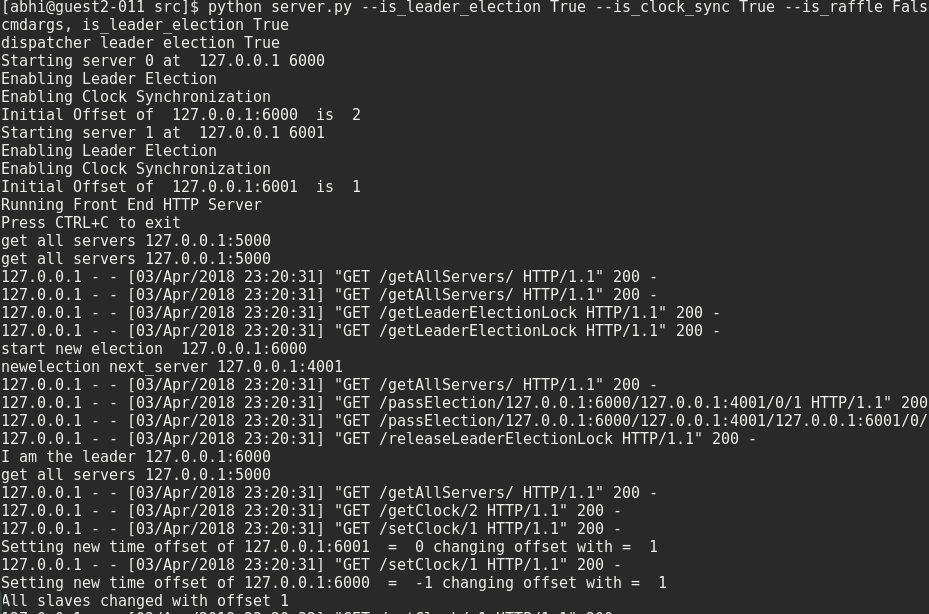
\includegraphics[width=\textwidth]{outputs/clock_sync_server.png}
        \caption{Leader Election and Clock Synchronization \label{fig:clong_synchronization}}
\end{figure}
\begin{figure}[H]
        \centering
        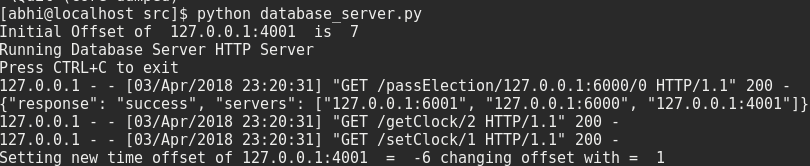
\includegraphics[width=\textwidth]{outputs/clock_sync_db.png}
        \caption{Leader Election and Clock Synchronization \label{fig:clong_synchronization}}
\end{figure}
\subsection{Totally Ordered Multicast}
This experiment is similar to the test case of totally ordered multicast.
Here, we create 2 front end servers and the databse server. 2 more clients
are created, which are registered on different servers. These clients
continuously send several requests to their respective servers.
Every 100th requests is stored in raffle, and after some time raffle 
winner is randomly selected.

\begin{figure}[H]
        \centering
        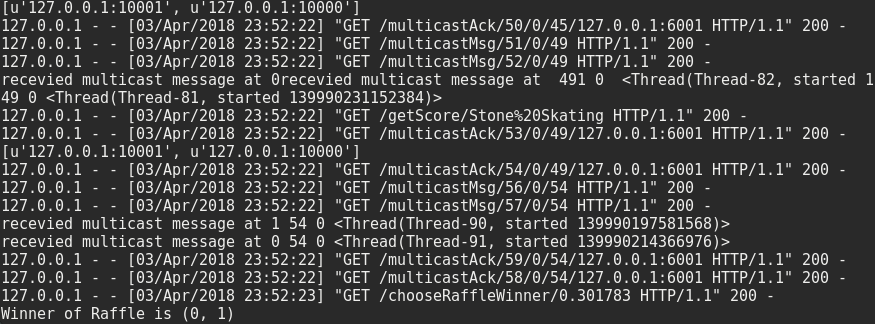
\includegraphics[width=\textwidth]{outputs/raffle_winner.png}
        \caption{Raffle Winner}
\end{figure}
\end{document}
